\documentclass[a4paper, 12pt]{article}

\usepackage[portuguese]{babel}
\usepackage[utf8]{inputenc}
\usepackage[T1]{fontenc}
\usepackage{amsmath}
\usepackage{url}
\usepackage{amssymb}
\usepackage{booktabs}
\usepackage{tikz}

\usepackage{graphicx}
\usepackage{caption}
\usepackage{subcaption}

\graphicspath{{../img/}}

\newcommand{\rom}[1]{\uppercase\expandafter{\romannumeral #1\relax}}

\linespread{1.25}

\begin{document}

\begin{titlepage}
    \centering
    \vspace*{4cm}
    \textbf{\huge{Classificando Tweets -- MAC5832}}\\

    \vskip 1cm

    Pedro Henrique Rocha Bruel

    \emph{phrb@ime.usp.br}

    \emph{nUSP: 7143336}

    \vfill
    \normalsize{\emph{DCC - IME\\
    Universidade de São Paulo}\\}
    \normalsize{São Paulo, \today}
\end{titlepage}

\section{Introdução} \label{sec:intro}

Este relatório apresenta visualizações e algoritmos de aprendizado de máquina
utilizados no primeiro \textit{dataset} da disciplina \textbf{MAC5832}.

O \textit{dataset} consiste de um conjunto de \textit{tweets} sobre companhias
aéreas, associado a avaliações de \textit{sentimento}.  Os algoritmos de
aprendizado de máquina implementados foram o \textit{Perceptron} e o
\textit{Gradient Descent}. Os dois algoritmos estão descritos nas Seções
\ref{sec:percep} e \ref{sec:gd}.  Visualizações do \textit{dataset} são
apresentadas na Seção \ref{sec:viz}. A Seção \ref{sec:concl} discute os
resultados e conclui este relatório.

\subsection{Estrutura de Diretórios}

Os diretórios deste trabalhos estão organizados da
seguinte forma:

\paragraph{\texttt{./doc}} Contém os arquivos necessários
para gerar este documento.

\paragraph{\texttt{./data}} Contém os conjuntos de dados
disponibilizados para treinamento e testes.

\paragraph{\texttt{./src}} Contém o código implementado
para o \textit{Perceptron} e \textit{Gradient Descent}.

\paragraph{\texttt{./src/plot}} Contém o código para
gerar as figuras com as visualizações, e também as figuras.

\section{Algoritmos de Aprendizado de Máquina}

Esta Seção discute os algoritmos de aprendizado de máquina
e suas implementações, feitas em \texttt{Python 3} e usando os
módulos \texttt{nltk}, \texttt{sklearn}, \texttt{numpy},
\texttt{csv} e \texttt{re}.

Utilizei o tutorial sobre \textit{Bag of
Words}\footnote{\url{https://www.kaggle.com/c/word2vec-nlp-tutorial/details/part-1-for-beginners-bag-of-words}},
disponibilizado na página da Tarefa \rom{1}, para gerar um \textit{vocabulário}
com as palavras mais frequentes nos \textit{tweets} do \textit{dataset}.

O vocabulário foi então usado para gerar os \textit{vetores de características}
utilizados para treinar os algoritmos e realizar as predições.
Os vetores de características contêm um \texttt{1} na posição
correspondente a uma determinada palavra se o \textit{tweet}
contém aquela palavra, e um \texttt{0} caso contrário.

Além disso, cada vetor de características é inicializado com
um \texttt{1} na primeira posição, correspondente ao
\textit{threshold} do classificador.

\subsection{Perceptron} \label{sec:percep}

Considere um vetor $\boldsymbol{w}$ de pesos inicializado com $N + 1$
\texttt{1}s, onde cada peso $w_i, 0 \leq i \leq N$ corresponde a uma
característica dos vetores de características dos \textit{tweets} do
\textit{dataset}, e $N$ é o número de características extraídas do conjunto.

A cada passo do algoritmo \textit{Perceptron}, vamos calcular a classificação
$c_j$ de cada um dos $M$ vetores $\boldsymbol{x}_j, 0 \leq j \leq M$ de características
usando a seguinte equação:

\begin{align*}
    c_j = step\bigg(\sum_{i = 0}^{N}{w_i\boldsymbol{x}_{j}^{i}}\bigg) = step\bigg(\boldsymbol{w}^{T}\boldsymbol{x}_j\bigg)
\end{align*}

Onde a função $step$ é dada por:

\begin{align*}
    step(y) = \begin{cases}
        1 & \text{ se } y \geq 0 \\
        -1 & \text{ caso contrário.}
    \end{cases}
\end{align*}

Depois, para cada vetor $\boldsymbol{x}_j, 0 \leq j \leq M$ vamos atualizar o vetor
$\boldsymbol{w}$ de pesos da seguinte maneira:

\begin{align*}
    \boldsymbol{w} = \boldsymbol{w} + \alpha\boldsymbol{x}_j(z_j - c_j)
\end{align*}

Aqui, $\boldsymbol{x}_j$ é um vetor de características, $\alpha$ é a
\textit{taxa de aprendizado}, $z_j$ é a classificação correta de
$\boldsymbol{x}_j$ e $c_j$ é a predição feita pelo algoritmo nessa iteração.

A minha implementação do \textit{Perceptron} executa esse procedimento para
todos os exemplos no conjunto de testes até que o número de exemplos
classificados erroneamente seja menor ou igual a um limite $\mu$. Nesse
\textit{dataset}, utilizei $\mu = 6$. Depois do treinamento do modelo, obtemos
um vetor $\boldsymbol{w}^{*}$, que é usado para gerar as predições para cada \textit{tweet}
contido nos dados para teste.

\subsection{Gradient Descent} \label{sec:gd}

Considere um vetor $\boldsymbol{w}$ de pesos inicializado
com $N + 1$ \texttt{1}s, onde cada peso $w_i,\: 0 \leq i \leq N$
corresponde a uma característica dos vetores de características
dos \textit{tweets} do \textit{dataset}, e $N$ é o número
de características extraídas do conjunto.

A cada passo do algoritmo \textit{Gradient Descent}, vamos calcular a
classificação $c_j$ de todos os vetores $\boldsymbol{x}_j,\: 0 \leq j \leq M,\: \boldsymbol{x}_j \in
\boldsymbol{X}$ de características, onde $\boldsymbol{X}$ é a matriz
de exemplos. Faremos a classificação usando a seguinte equação:

\begin{align*}
    \boldsymbol{C} = \boldsymbol{w}^{T}\boldsymbol{X}
\end{align*}

Aqui, $\boldsymbol{C}$ é um vetor contendo um \textit{valor real} para
cada exemplo $\boldsymbol{x}_j \in \boldsymbol{X}$. Para obter uma predição
da classificação de algum $\boldsymbol{x}_j$, usamos função $step(\boldsymbol{C}_j)$,
onde $\boldsymbol{C}_j$ é $j$-ésimo valor em $\boldsymbol{C}$. A função $step$
é, novamente, dada por:

\begin{align*}
    step(y) = \begin{cases}
        1 & \text{ se } y \geq 0 \\
        -1 & \text{ caso contrário.}
    \end{cases}
\end{align*}

Depois de calcular $\boldsymbol{C}$,  atualizamos o vetor $\boldsymbol{w}$
de pesos da seguinte maneira:

\begin{align*}
    \boldsymbol{w} = \boldsymbol{w} - \alpha \frac{1}{M} \boldsymbol{X}(\boldsymbol{C} - \boldsymbol{Z})
\end{align*}

Aqui, $\boldsymbol{X}$ é a matriz de exemplos, $\alpha$ é a \textit{taxa de
aprendizado}, $\boldsymbol{Z}$ é a matriz com as classificações corretas de
cada exemplo em $\boldsymbol{X}$ e $\boldsymbol{C}$ é a matriz de predições
feita pelo algoritmo nessa iteração.

A minha implementação do \textit{Gradient Descent} executa esse procedimento
até que o número de iterações seja maior do que um limite $\rho$. Nesse
\textit{dataset}, utilizei $\rho = 500$. Depois do treinamento do modelo,
obtemos um vetor $\boldsymbol{w}^{*}$, que é usado para gerar as predições para cada
\textit{tweet} contido nos dados para teste.

\section{Resultados}

\begin{figure}[htpb]
    \centering
    \begin{subfigure}[htpb]{0.45\textwidth}
        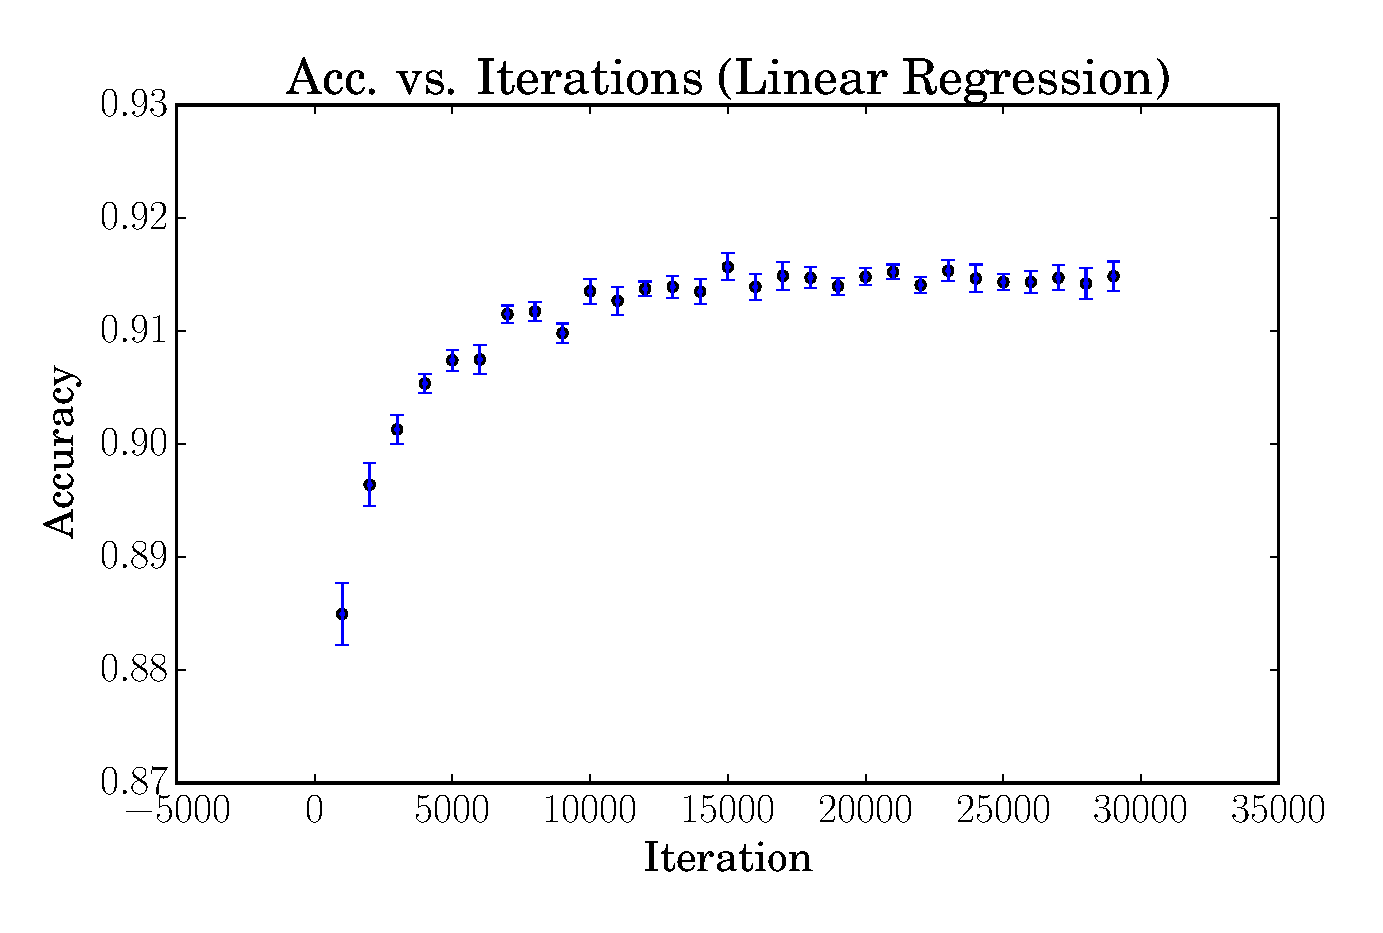
\includegraphics[width=\textwidth]{acc_vs_iterations_linreg}
        \caption{}
        \label{fig:snt}
    \end{subfigure}
    %add desired spacing between images, e. g. ~, \quad, \qquad, \hfill etc.
    %(or a blank line to force the subfigure onto a new line)
    \begin{subfigure}[htpb]{0.45\textwidth}
        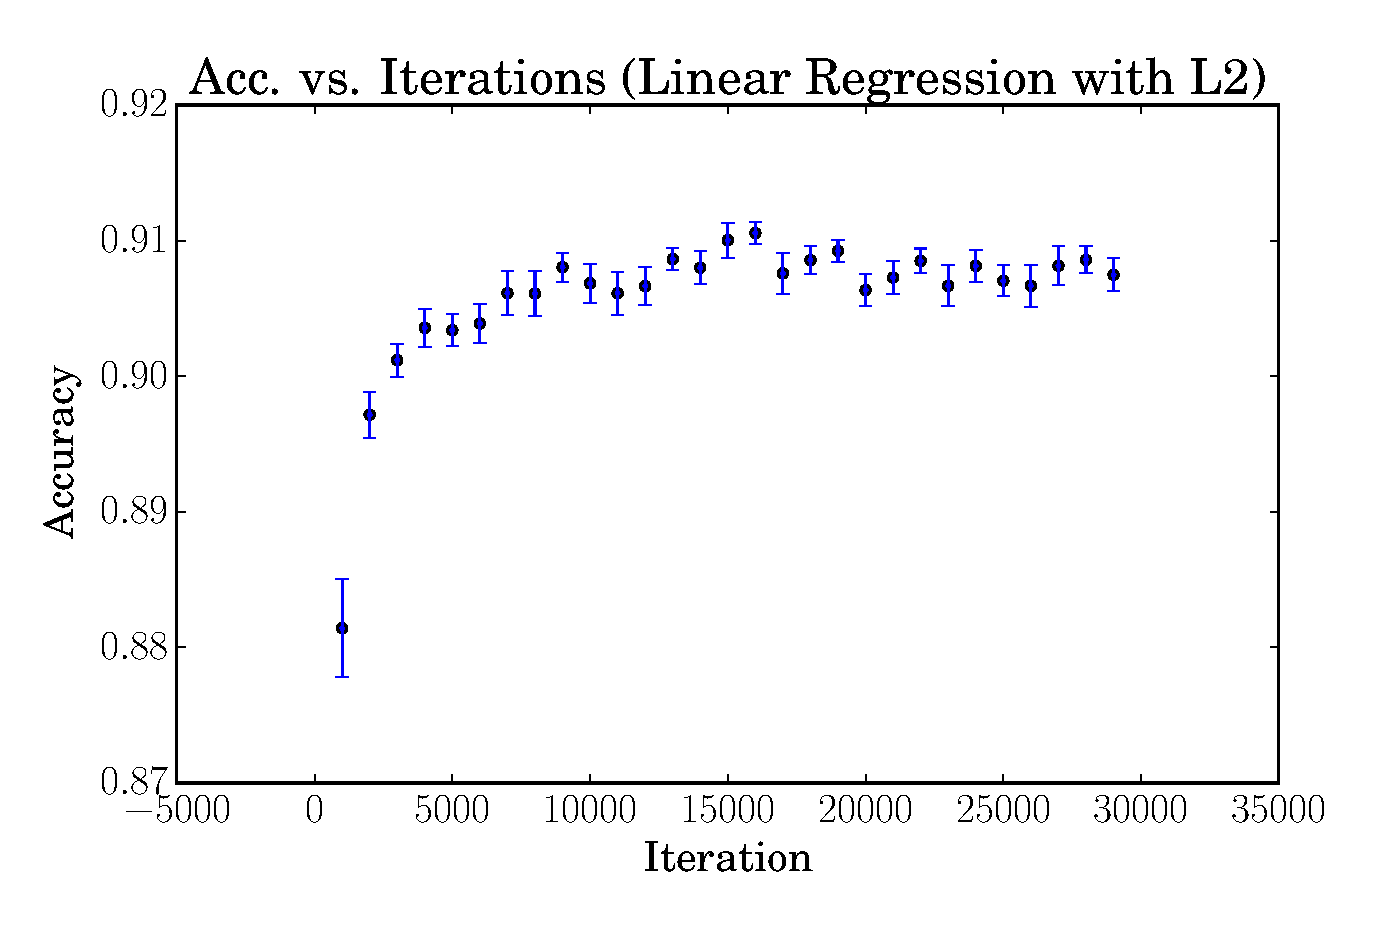
\includegraphics[width=\textwidth]{acc_vs_iterations_linregL2}
        \caption{}
        \label{fig:ret}
    \end{subfigure}
    \hfill %add desired spacing between images, e. g. ~, \quad, \qquad, \hfill etc.
    %(or a blank line to force the subfigure onto a new line)
    \begin{subfigure}[htpb]{0.45\textwidth}
        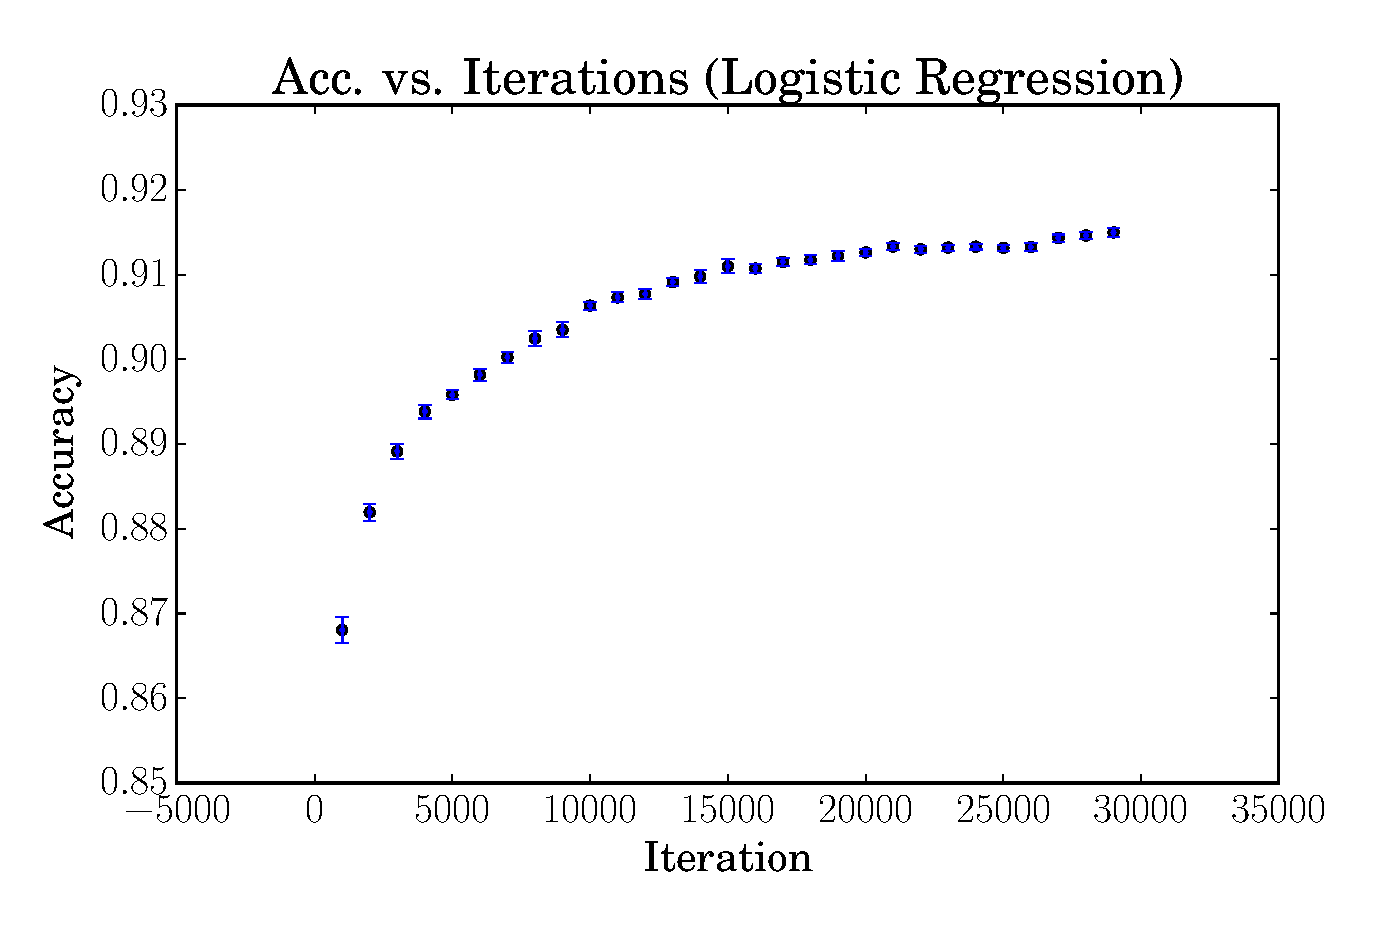
\includegraphics[width=\textwidth]{acc_vs_iterations_logreg}
        \caption{}
        \label{fig:gwd}
    \end{subfigure}
    %add desired spacing between images, e. g. ~, \quad, \qquad, \hfill etc.
    %(or a blank line to force the subfigure onto a new line)
    \begin{subfigure}[htpb]{0.45\textwidth}
        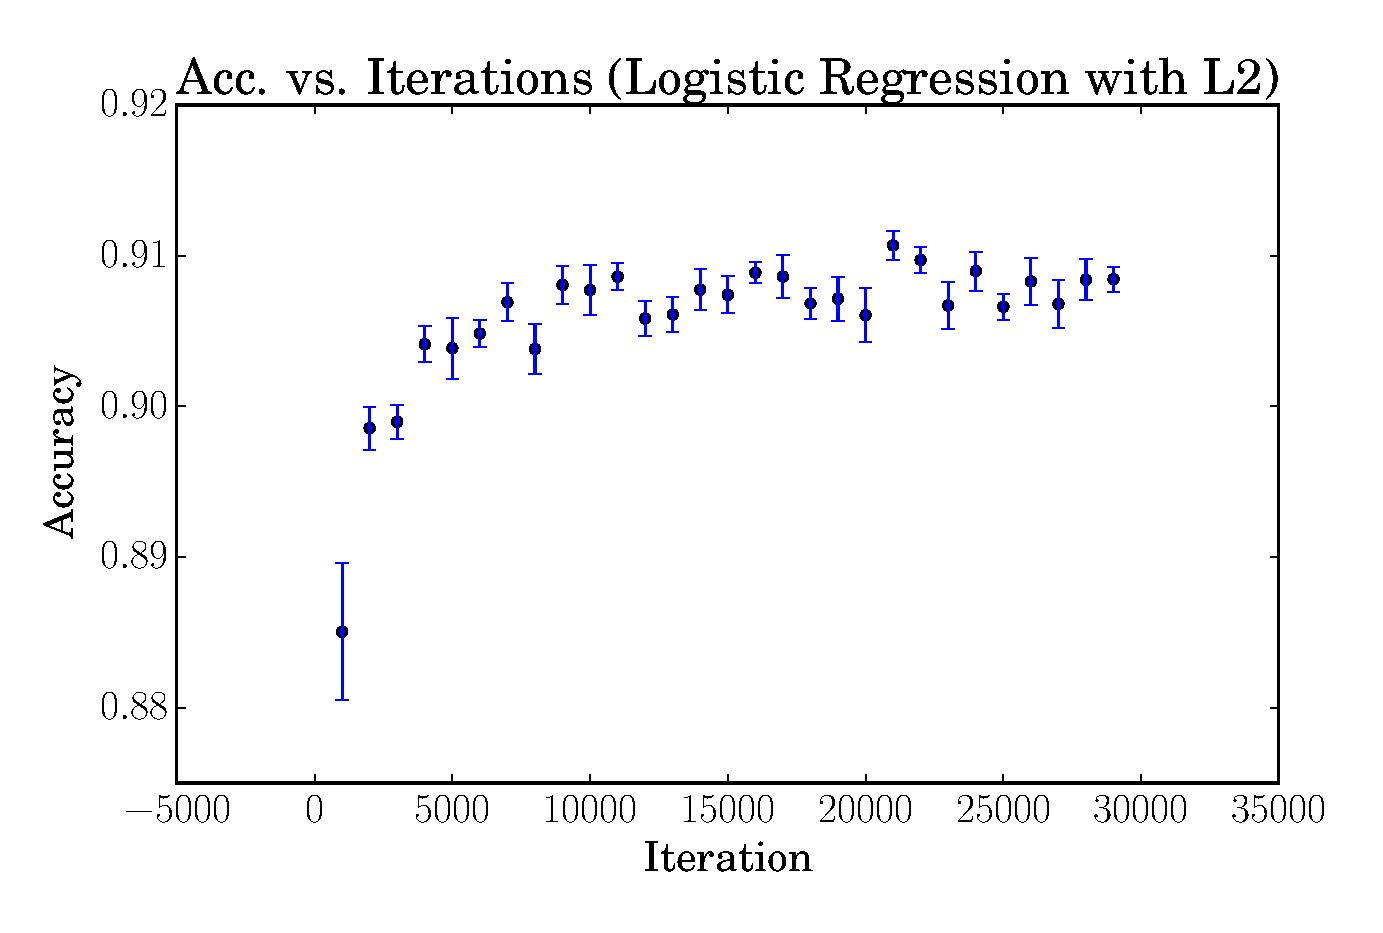
\includegraphics[width=\textwidth]{acc_vs_iterations_logregL2}
        \caption{}
        \label{fig:bwd}
    \end{subfigure}
    \caption{}\label{fig:viz}
\end{figure}

\begin{figure}[htpb]
    \centering
    \begin{subfigure}[htpb]{0.45\textwidth}
        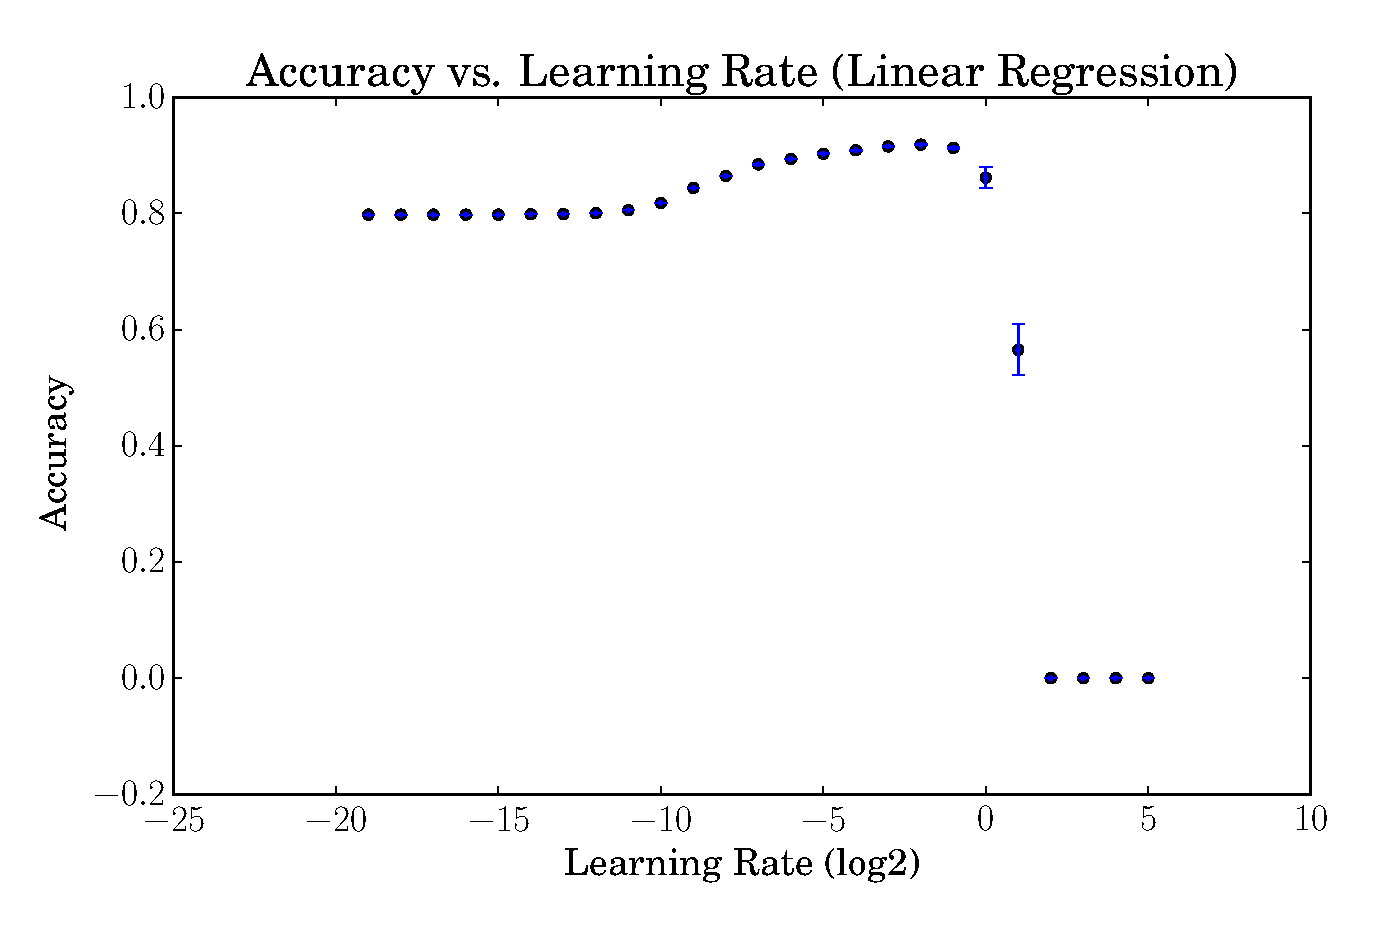
\includegraphics[width=\textwidth]{acc_vs_rate_linreg}
        \caption{}
        \label{fig:snt}
    \end{subfigure}
    %add desired spacing between images, e. g. ~, \quad, \qquad, \hfill etc.
    %(or a blank line to force the subfigure onto a new line)
    \begin{subfigure}[htpb]{0.45\textwidth}
        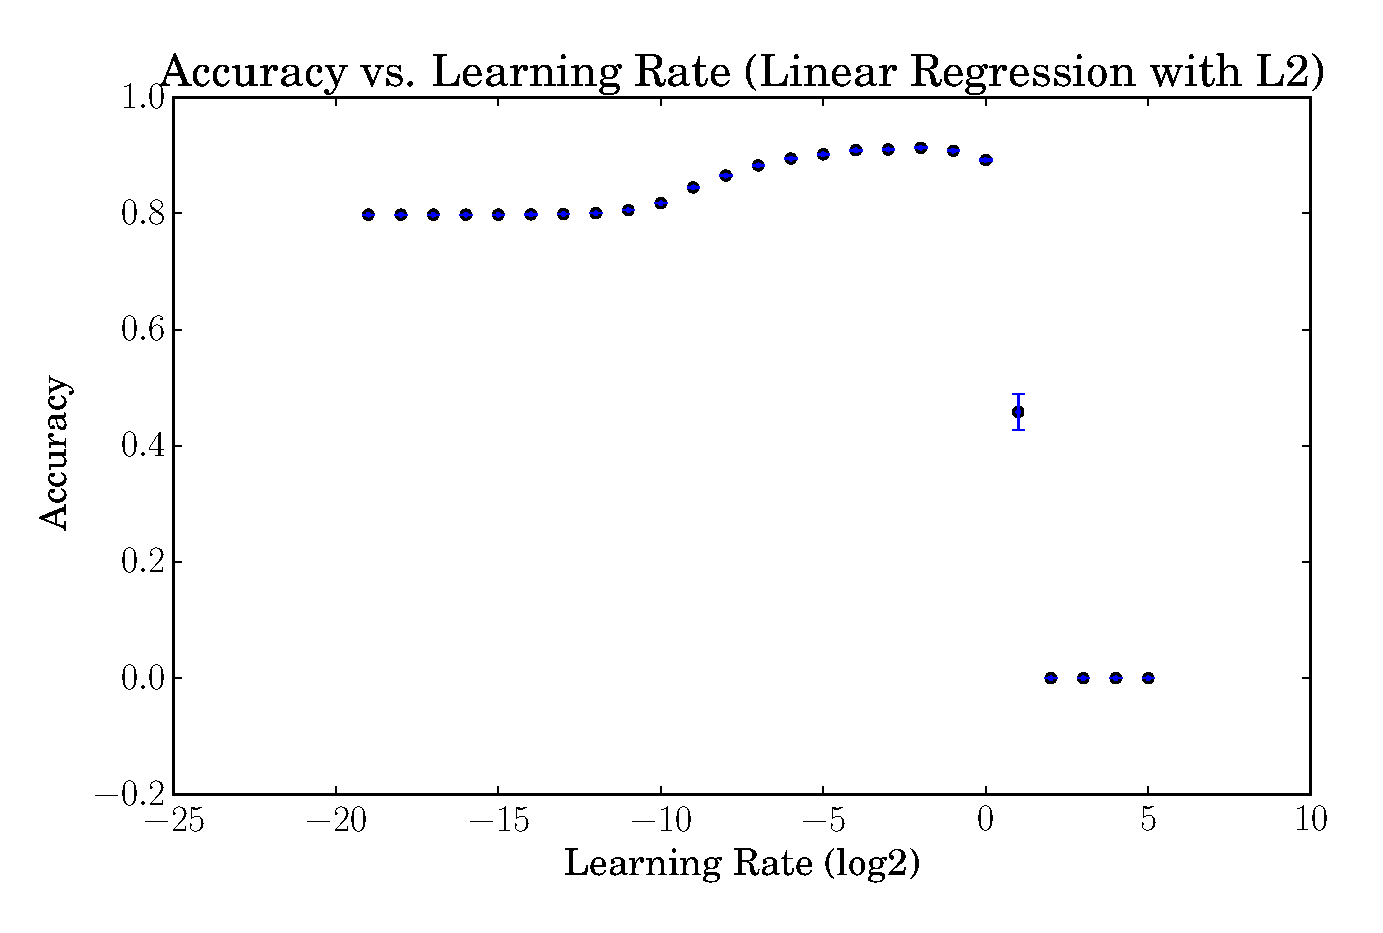
\includegraphics[width=\textwidth]{acc_vs_rate_linregL2}
        \caption{}
        \label{fig:ret}
    \end{subfigure}
    \hfill %add desired spacing between images, e. g. ~, \quad, \qquad, \hfill etc.
    %(or a blank line to force the subfigure onto a new line)
    \begin{subfigure}[htpb]{0.45\textwidth}
        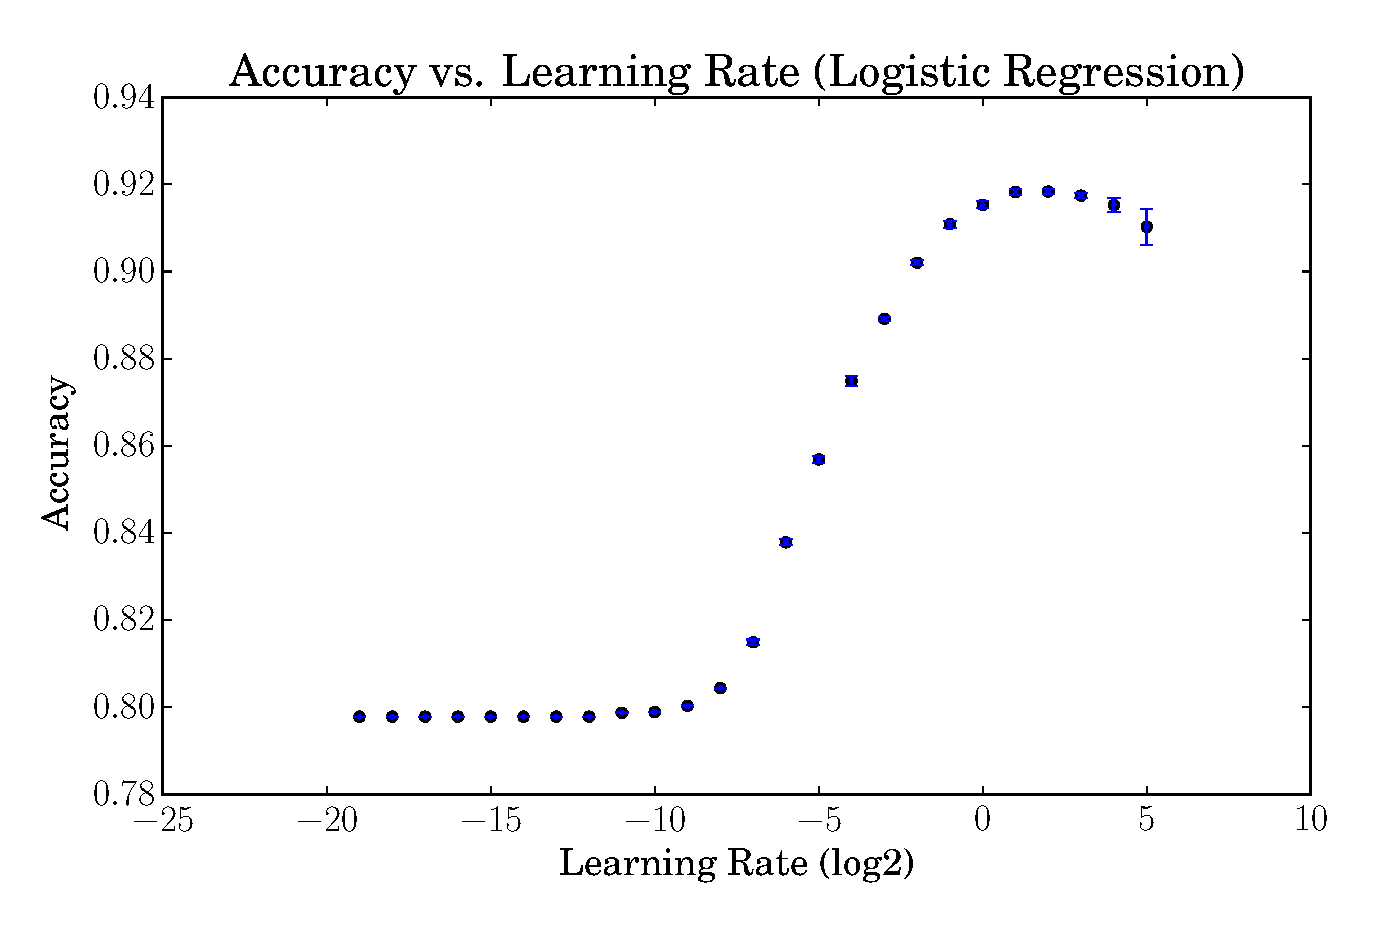
\includegraphics[width=\textwidth]{acc_vs_rate_logreg}
        \caption{}
        \label{fig:gwd}
    \end{subfigure}
    %add desired spacing between images, e. g. ~, \quad, \qquad, \hfill etc.
    %(or a blank line to force the subfigure onto a new line)
    \begin{subfigure}[htpb]{0.45\textwidth}
        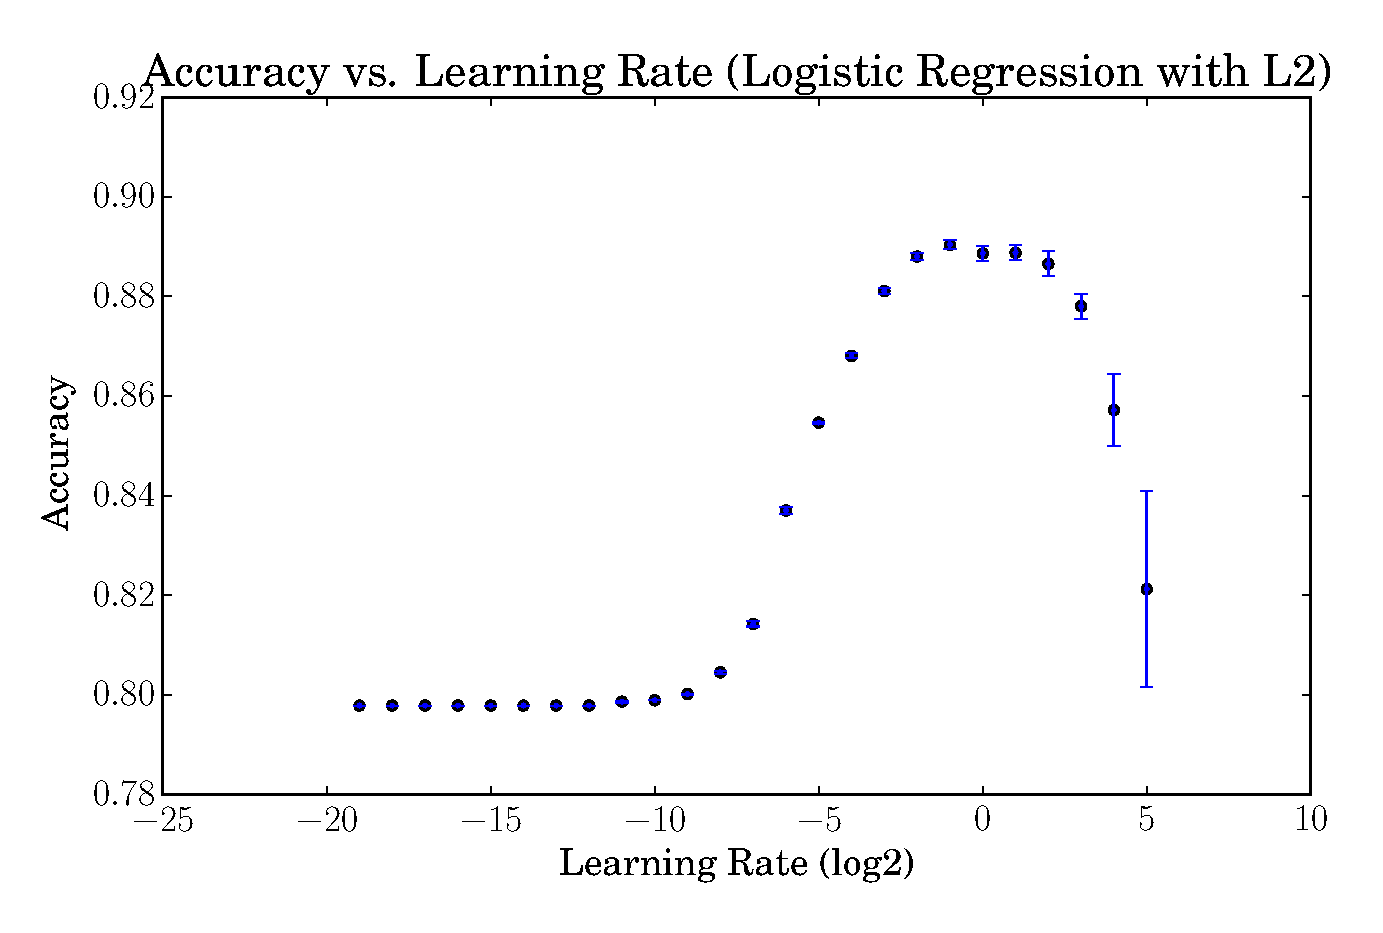
\includegraphics[width=\textwidth]{acc_vs_rate_logregL2}
        \caption{}
        \label{fig:bwd}
    \end{subfigure}
    \caption{}\label{fig:viz}
\end{figure}

\begin{figure}[htpb]
    \centering
    \begin{subfigure}[htpb]{0.45\textwidth}
        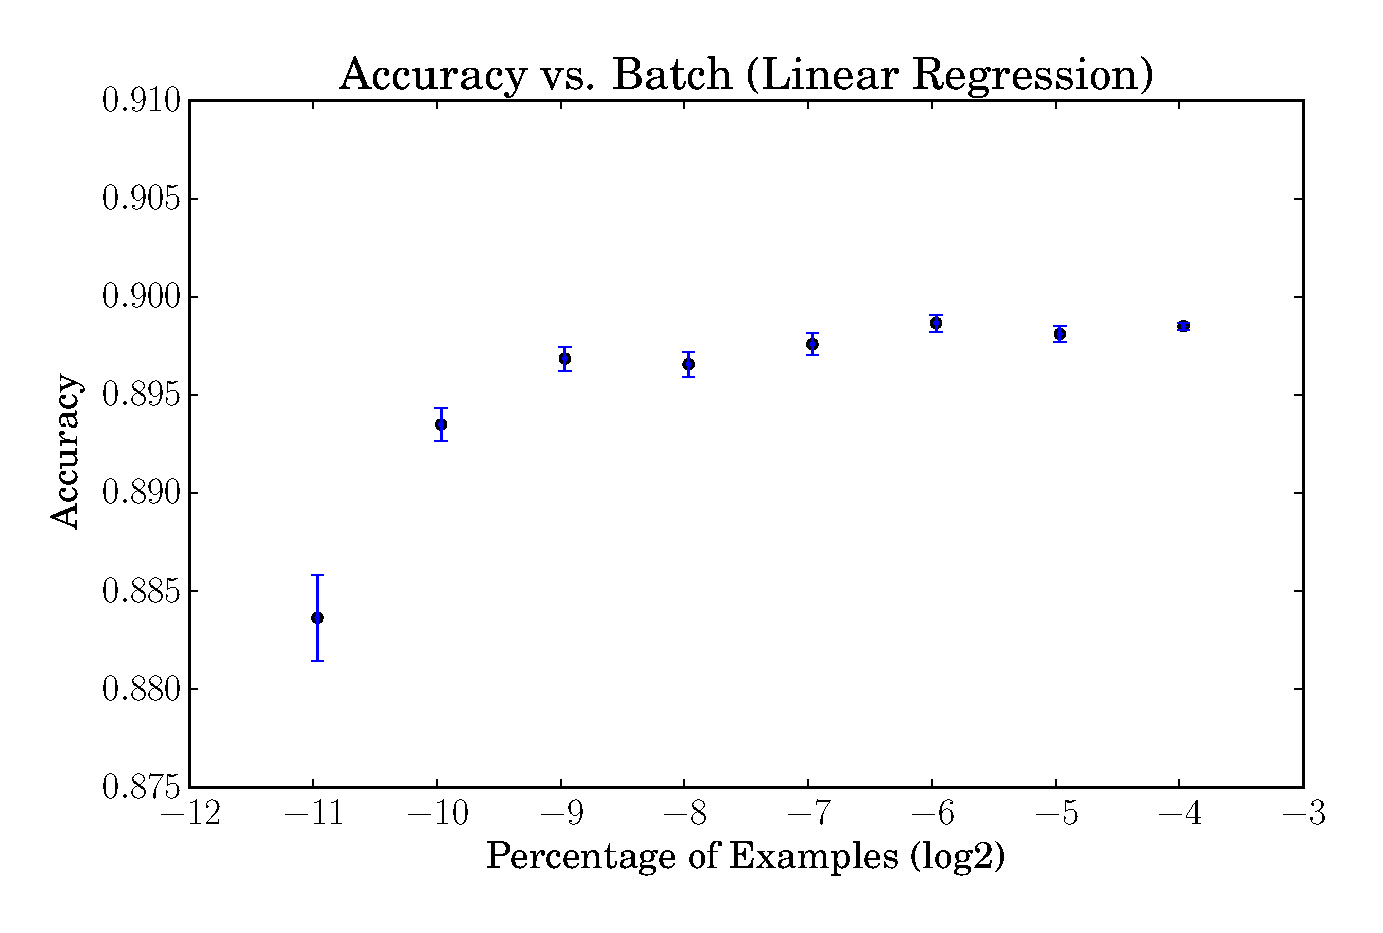
\includegraphics[width=\textwidth]{acc_vs_batchp_linreg}
        \caption{}
        \label{fig:snt}
    \end{subfigure}
    %add desired spacing between images, e. g. ~, \quad, \qquad, \hfill etc.
    %(or a blank line to force the subfigure onto a new line)
    \begin{subfigure}[htpb]{0.45\textwidth}
        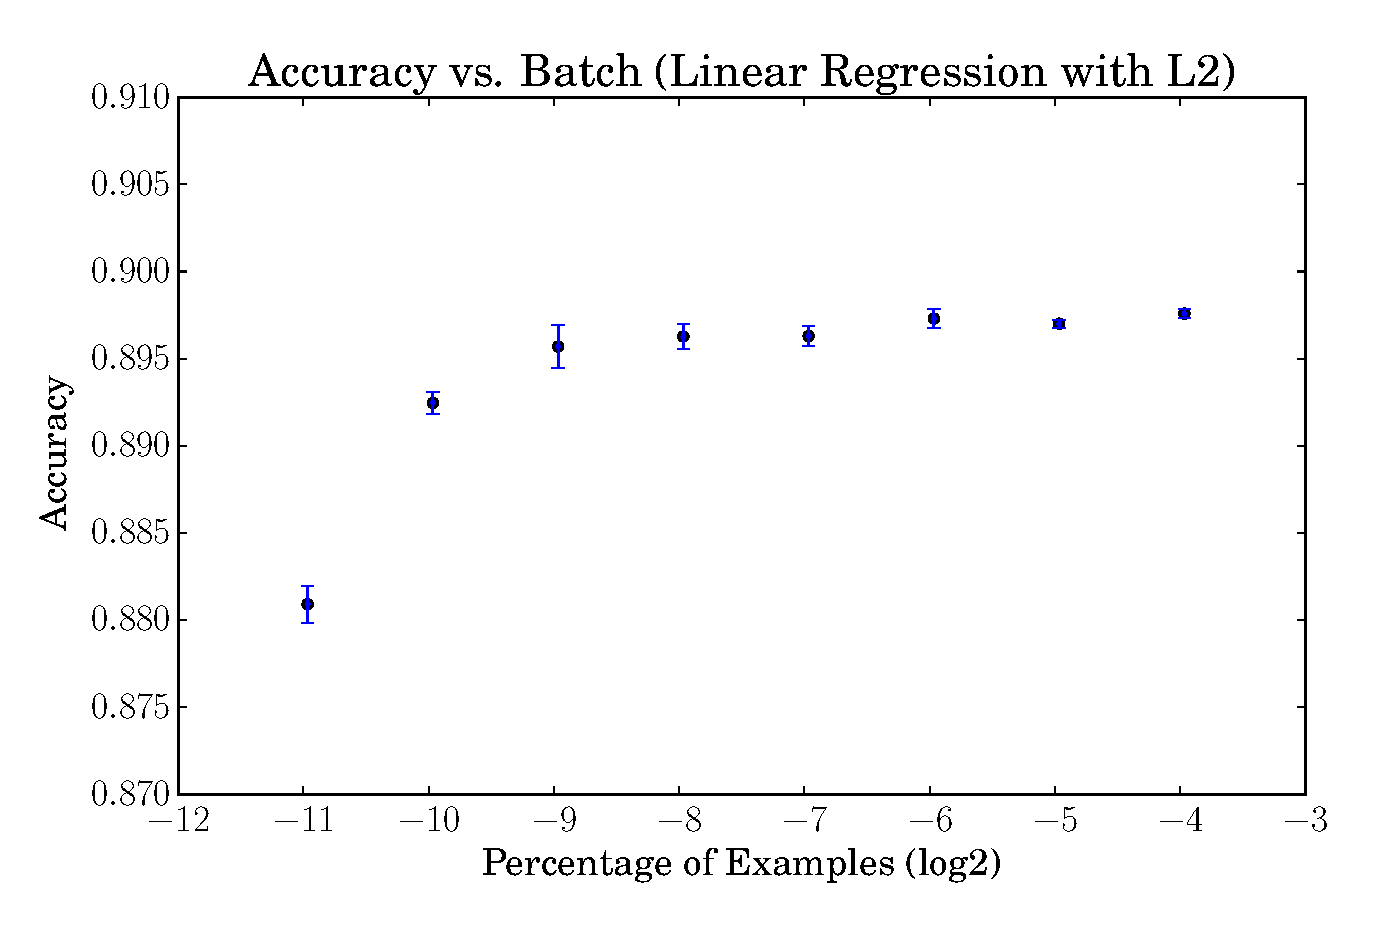
\includegraphics[width=\textwidth]{acc_vs_batchp_linregL2}
        \caption{}
        \label{fig:ret}
    \end{subfigure}
    \hfill %add desired spacing between images, e. g. ~, \quad, \qquad, \hfill etc.
    %(or a blank line to force the subfigure onto a new line)
    \begin{subfigure}[htpb]{0.45\textwidth}
        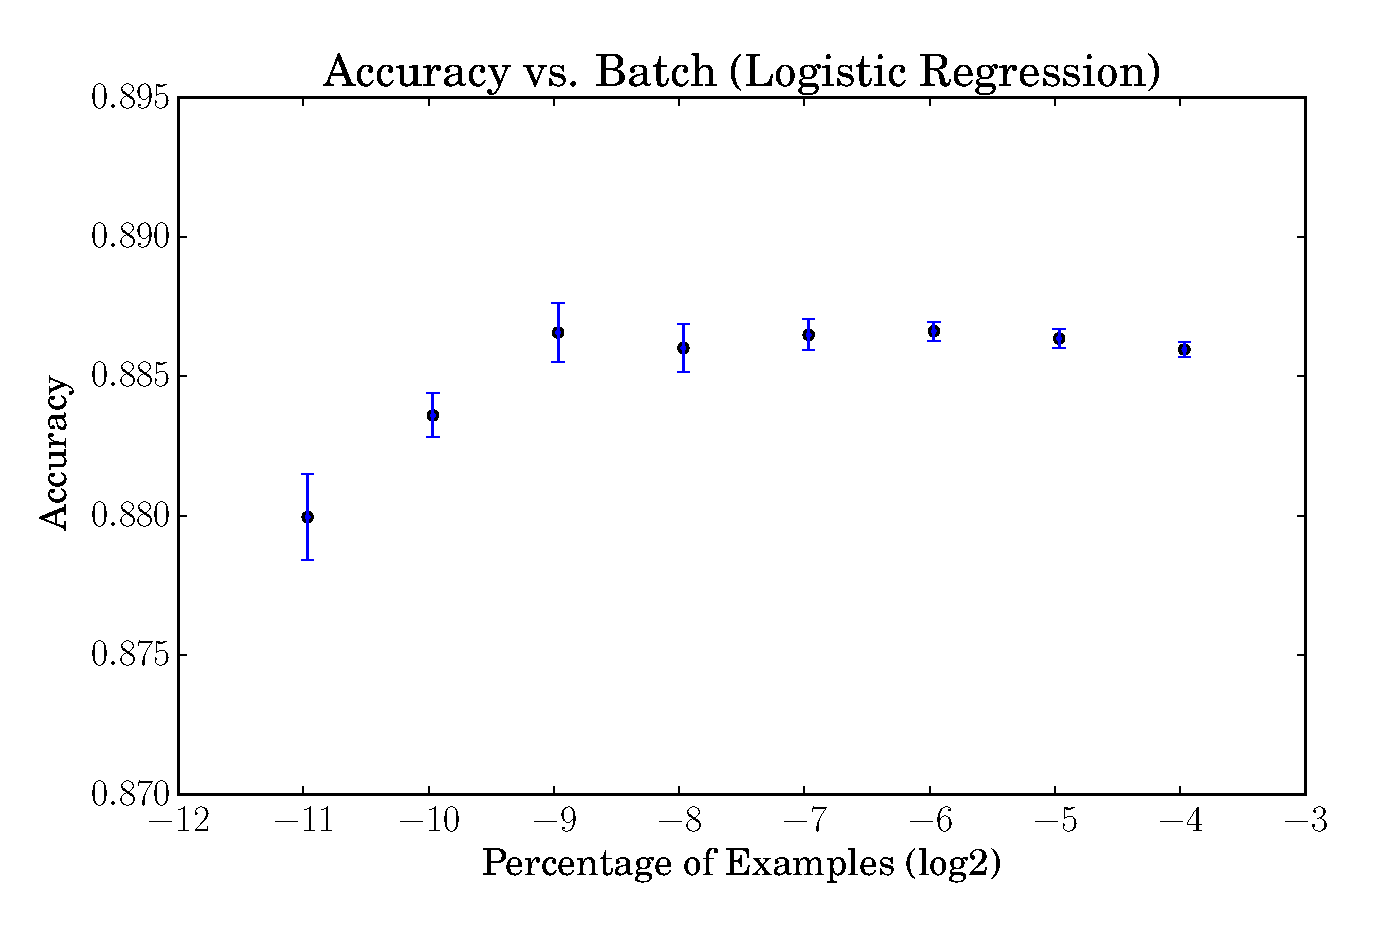
\includegraphics[width=\textwidth]{acc_vs_batchp_logreg}
        \caption{}
        \label{fig:gwd}
    \end{subfigure}
    %add desired spacing between images, e. g. ~, \quad, \qquad, \hfill etc.
    %(or a blank line to force the subfigure onto a new line)
    \begin{subfigure}[htpb]{0.45\textwidth}
        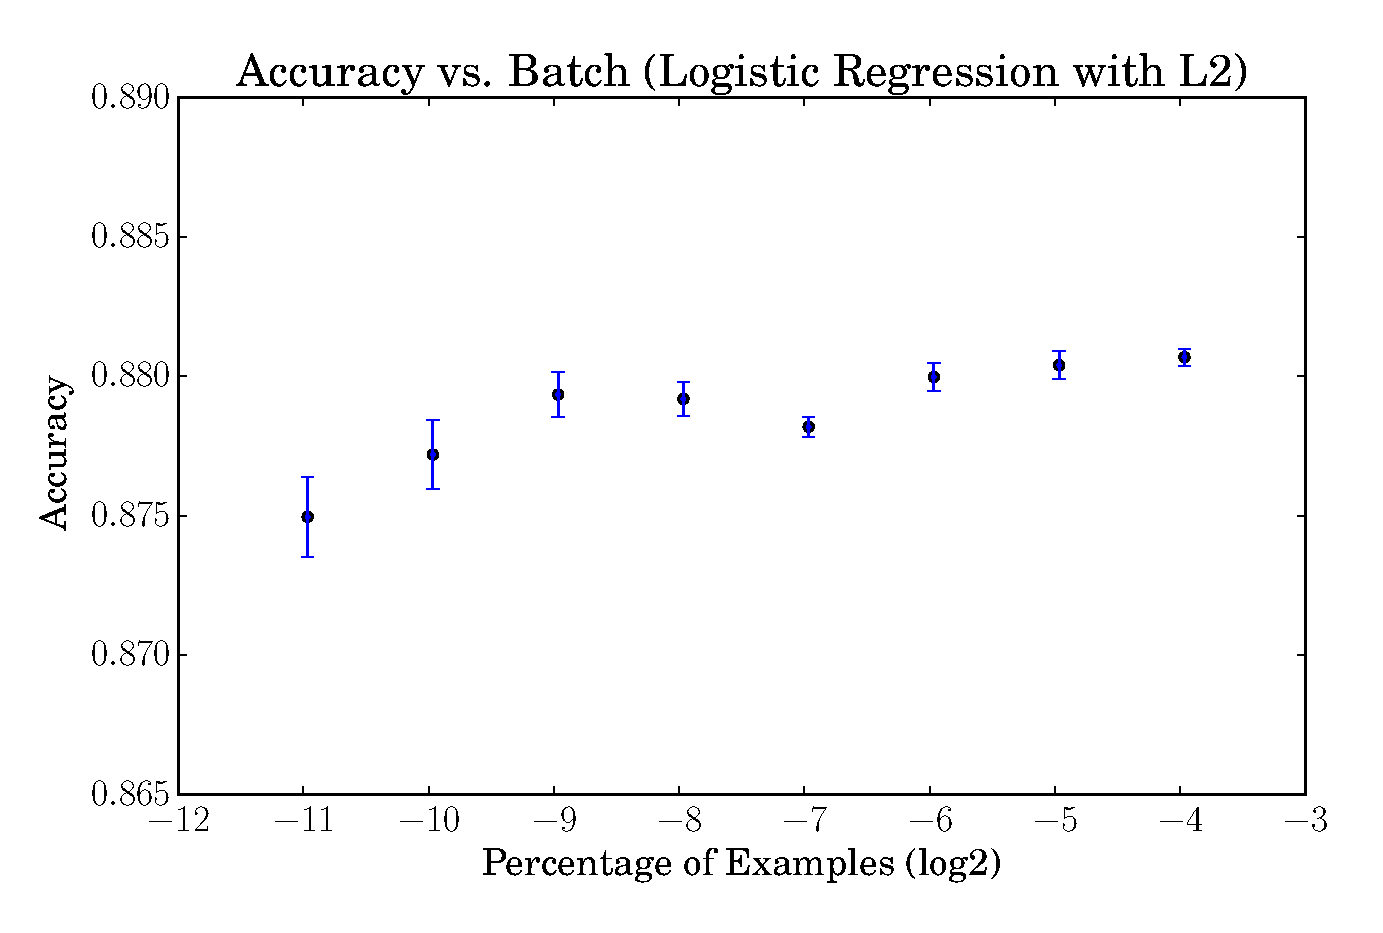
\includegraphics[width=\textwidth]{acc_vs_batchp_logregL2}
        \caption{}
        \label{fig:bwd}
    \end{subfigure}
    \caption{}\label{fig:viz}
\end{figure}

\begin{figure}[htpb]
    \centering
    \begin{subfigure}[htpb]{0.45\textwidth}
        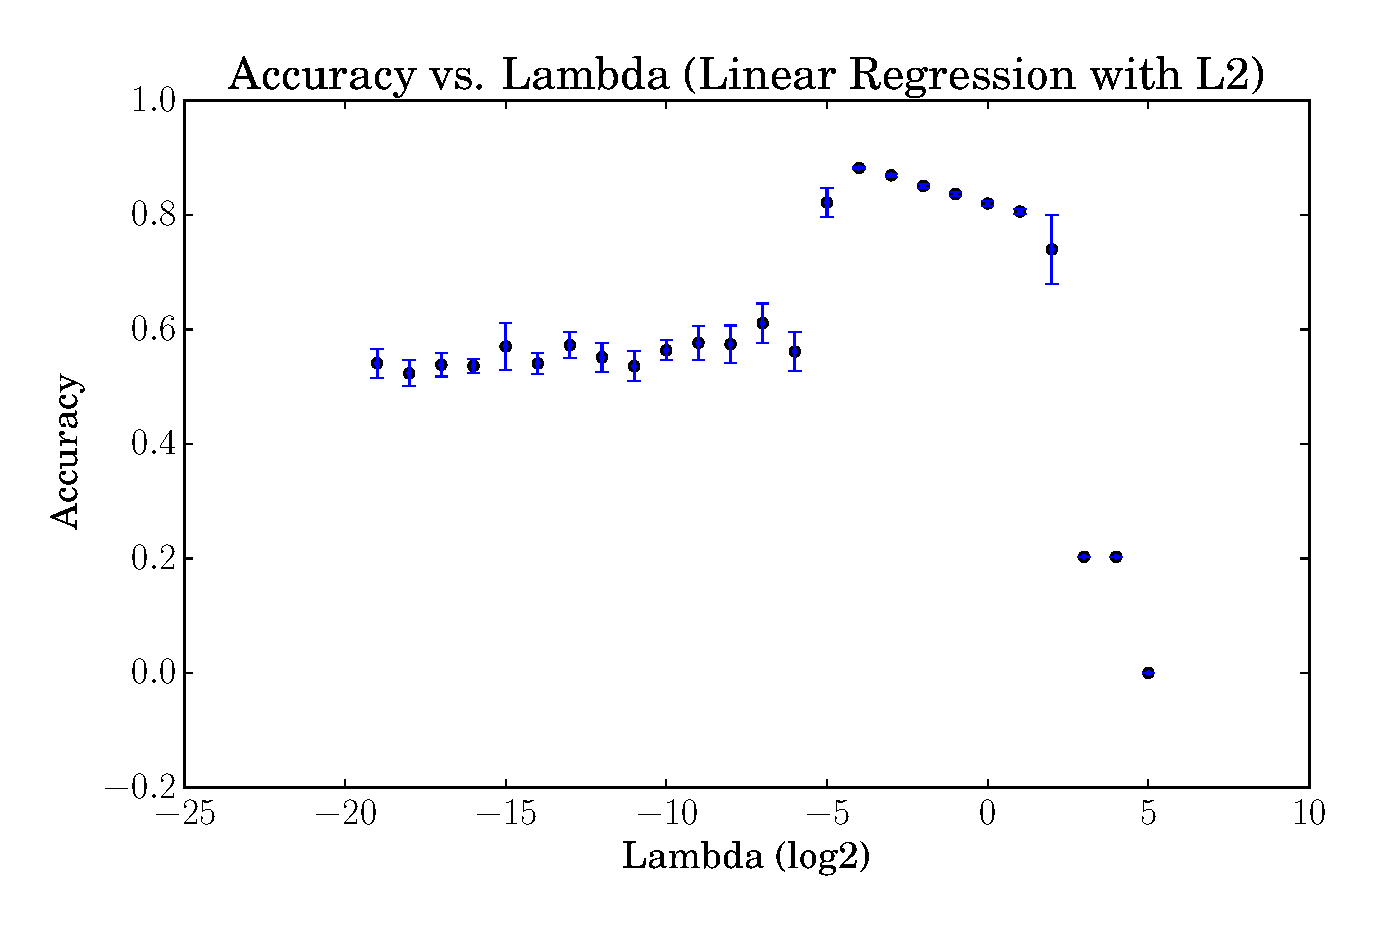
\includegraphics[width=\textwidth]{acc_vs_lambda_linregL2}
        \caption{}
        \label{fig:snt}
    \end{subfigure}
    %add desired spacing between images, e. g. ~, \quad, \qquad, \hfill etc.
    %(or a blank line to force the subfigure onto a new line)
    \begin{subfigure}[htpb]{0.45\textwidth}
        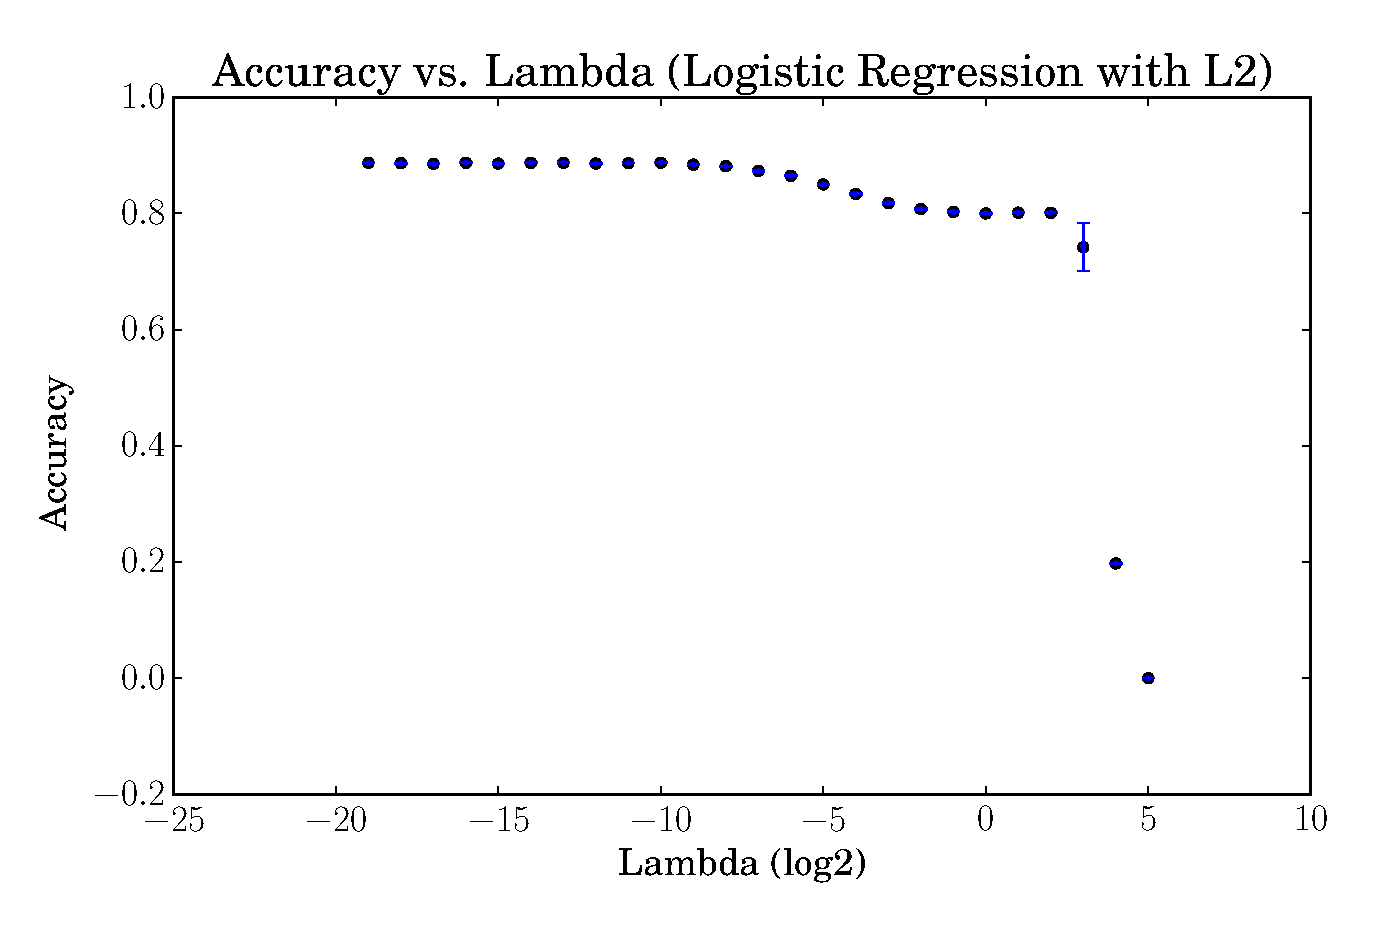
\includegraphics[width=\textwidth]{acc_vs_lambda_logregL2}
        \caption{}
        \label{fig:ret}
    \end{subfigure}
    \caption{}\label{fig:viz}
\end{figure}

\begin{figure}[htpb]
    \centering
    \begin{subfigure}[htpb]{0.45\textwidth}
        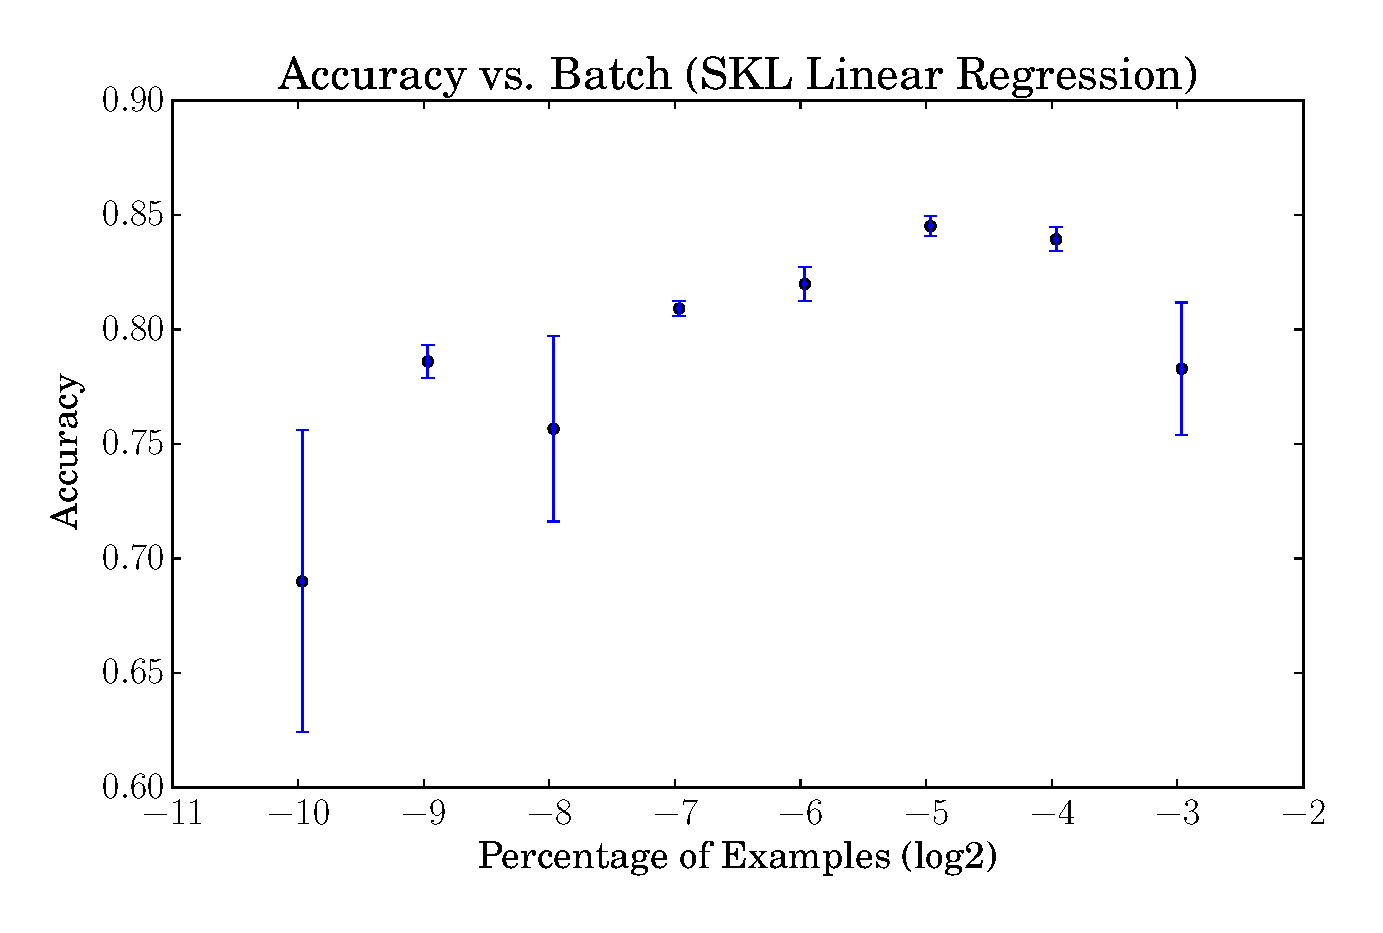
\includegraphics[width=\textwidth]{acc_vs_batchp_skl_linreg}
        \caption{}
        \label{fig:snt}
    \end{subfigure}
    %add desired spacing between images, e. g. ~, \quad, \qquad, \hfill etc.
    %(or a blank line to force the subfigure onto a new line)
    \begin{subfigure}[htpb]{0.45\textwidth}
        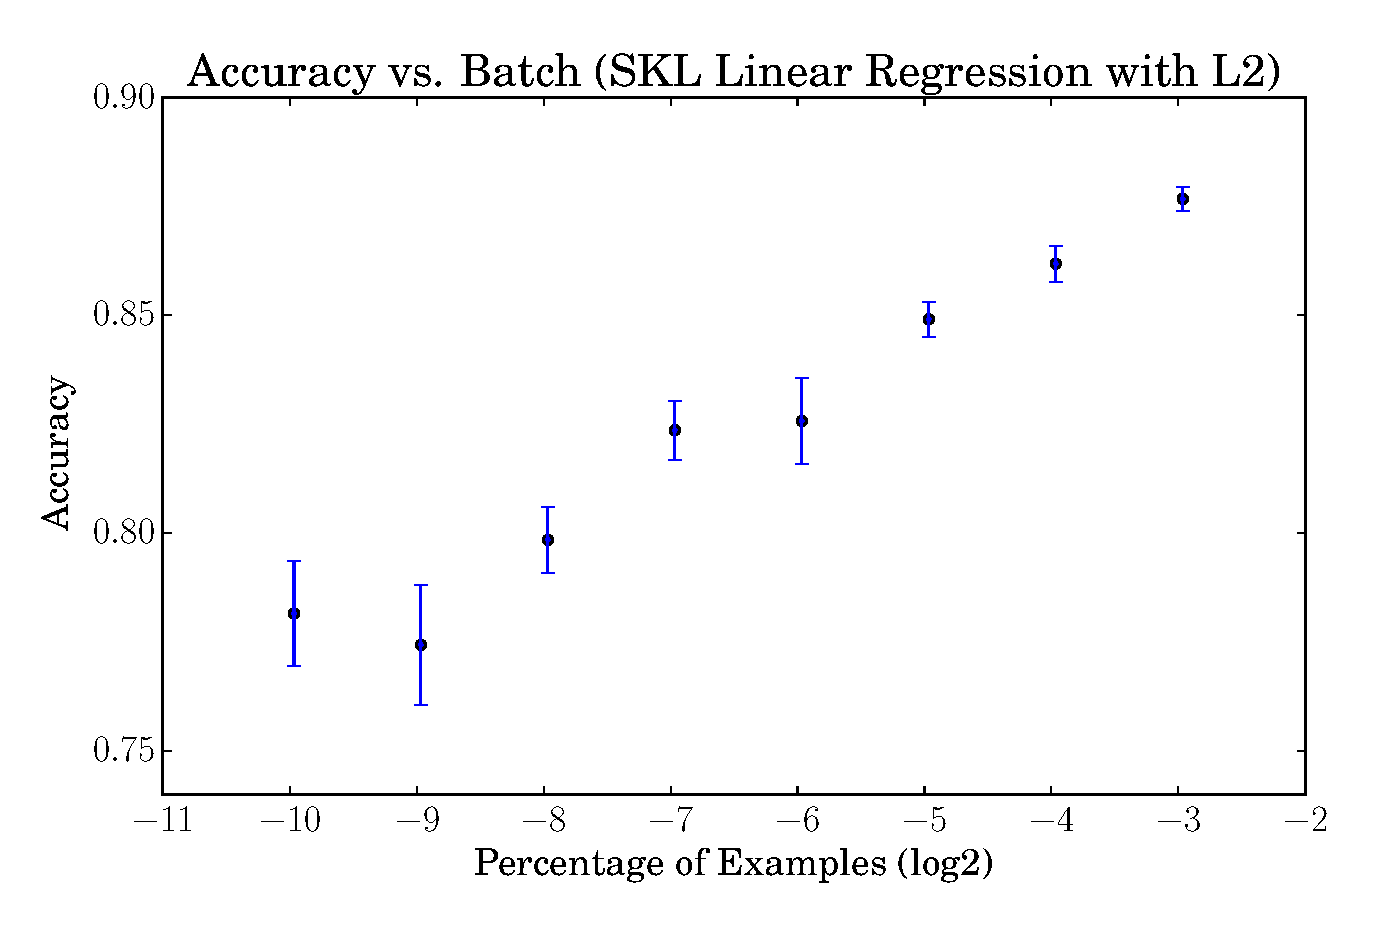
\includegraphics[width=\textwidth]{acc_vs_batchp_skl_linregL2}
        \caption{}
        \label{fig:ret}
    \end{subfigure}
    \hfill %add desired spacing between images, e. g. ~, \quad, \qquad, \hfill etc.
    %(or a blank line to force the subfigure onto a new line)
    \begin{subfigure}[htpb]{0.45\textwidth}
        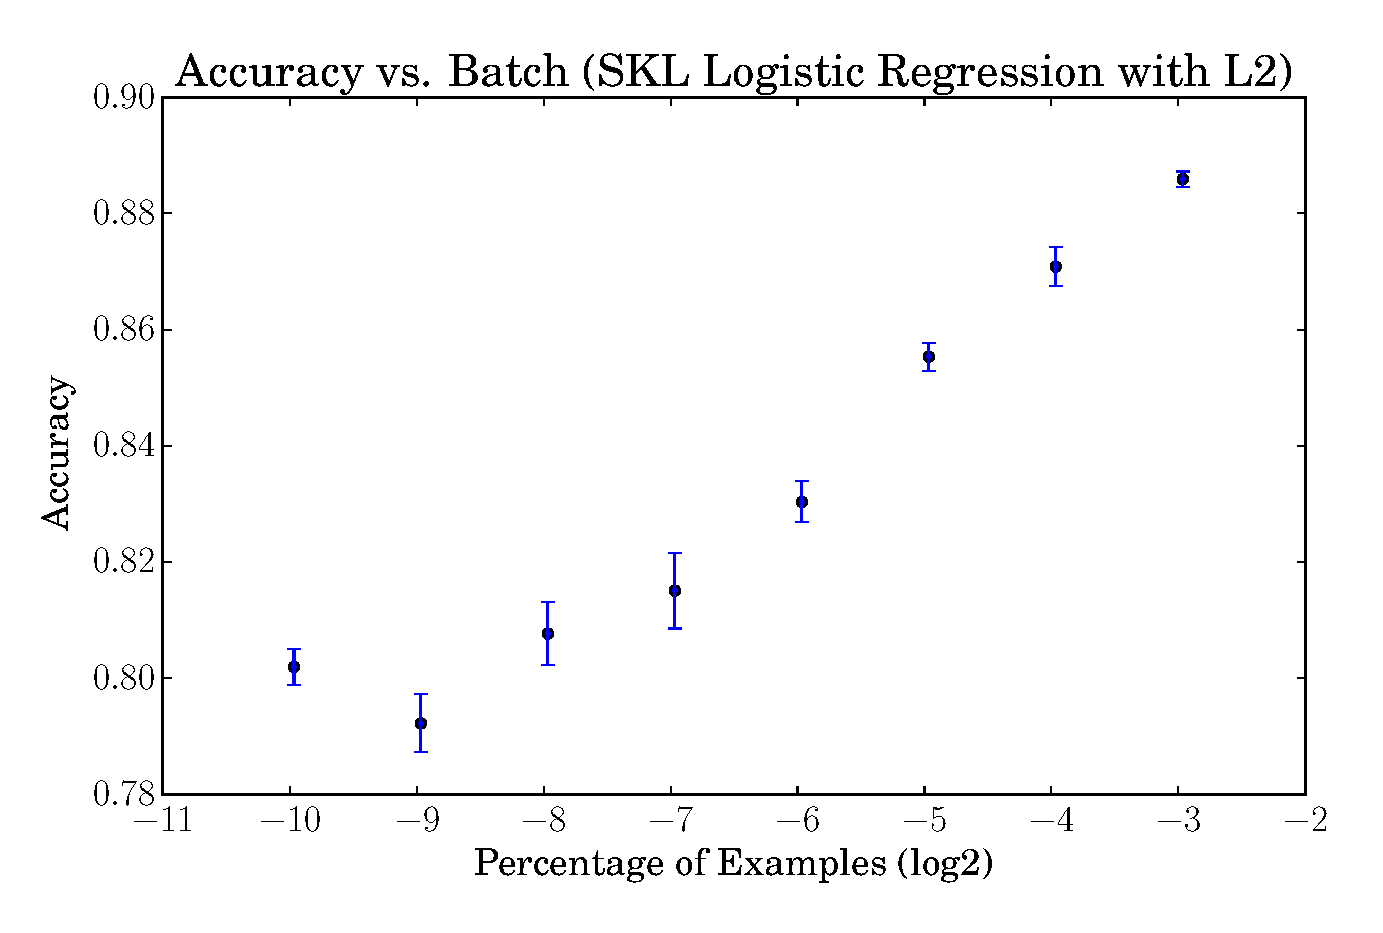
\includegraphics[width=\textwidth]{acc_vs_batchp_skl_logregL2}
        \caption{}
        \label{fig:gwd}
    \end{subfigure}
    \caption{}\label{fig:viz}
\end{figure}

\begin{figure}[htpb]
    \centering
    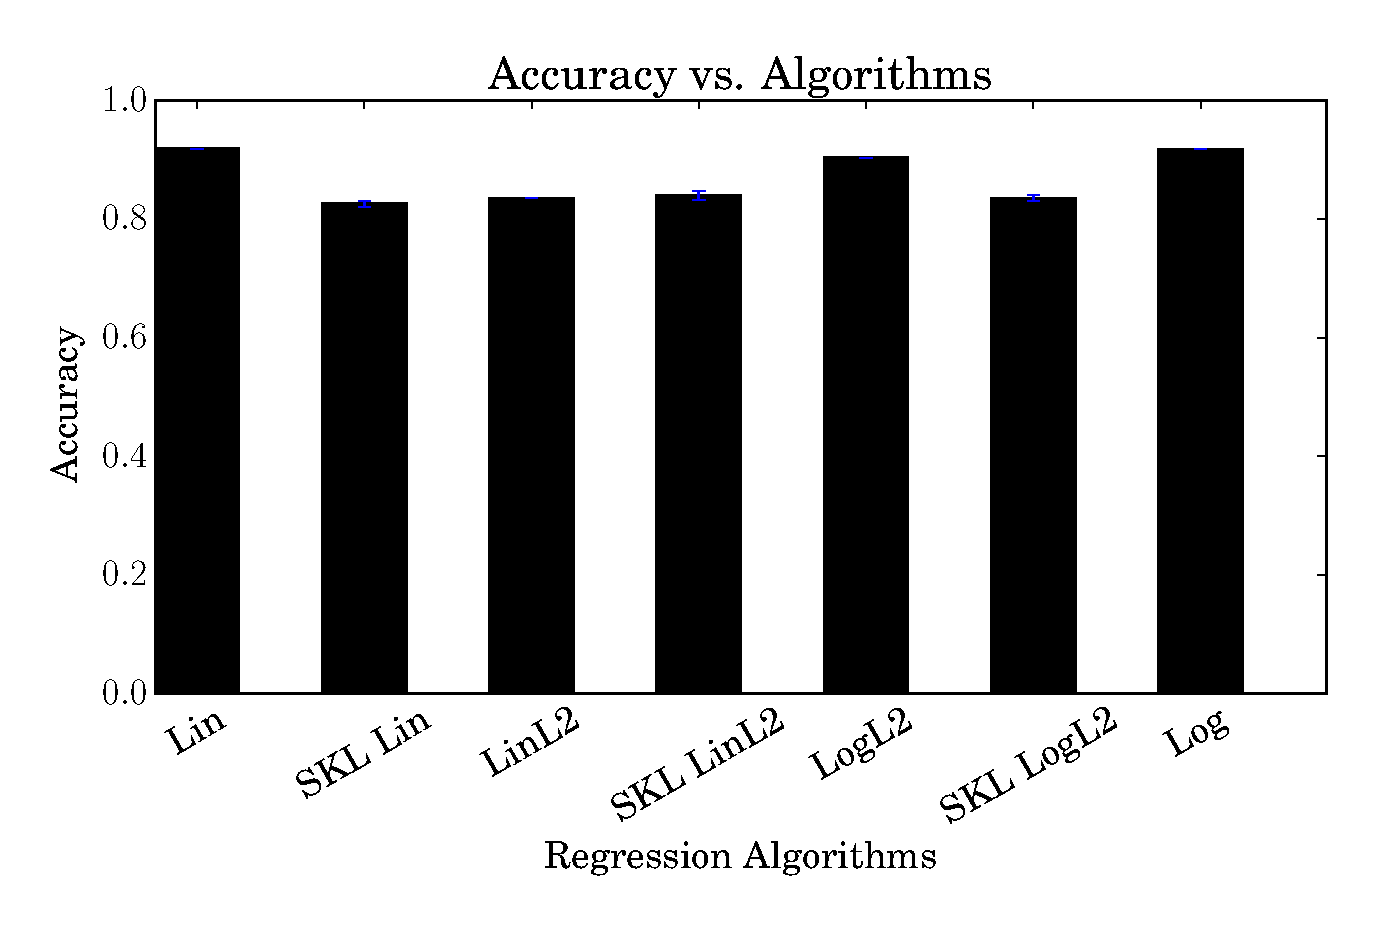
\includegraphics[width=.8\textwidth]{acc_vs_algorithm}
    \caption{}
    \label{fig:snt}
\end{figure}

\section{Conclusão} \label{sec:concl}

A minha implementação do \textit{Perceptron} teve um desempenho melhor do que a
implementação do \textit{Gradient Descent} mas, usando metade dos exemplos como
treinamento e outra metade como teste, ambos os algoritmos atingiram resultados
de por volta de $10\%$ de exemplos classificados erroneamente.

\end{document}
